\section{Test Harness}
\label{sec:harness}

% high level reference to test harness 
% is found in /src/doc/dev_guide/testing.tex

%%%%%%%%%%%%%%%%%%%%
% Test Harness Overview
The Test Harness is a flexible test control system intended to provide a thorough 
parameter space exploration of remapping and redistribution of distributed arrays and fields.
The parameter space is defined through configuration files which are interpreted at
run time to perform the desired tests.

The Test Harness is integrated into the Unit test framework, enabling
the Test Harness to be built and run as part of the Unit tests. The test results 
are reported to a single standard-out file which is located with the unit test 
results.

The motivation for employing such a hierarchy configuration files is to allow a 
high degree of customization of the test configurations by combining individual 
specification files. Complex combinations of test cases are easily specified in high level terms.
Each class will have its own collection of specification files tailored to the needs of that class.

\subsection{Specifying Test Harness Tests}
The test harness code consists of a single executable that uses a customizable configuration
files which are located within the \texttt{<classdir>/tests/harness\_config} directory of each 
supported class; currently only ESMF\_ARRAY and ESMF\_FIELD.

There are three ways to invoke the test harness, as an integral part of running unit
tests; as a stand-alone test invoked through gmake; and as a standalone test invoked through the command line.

Running the harness along with the unit tests provides
frequent regression testing of the redistribution and regridding features.  

Running the test harness
in stand alone mode using gmake is useful for isolating faults in failed test cases.  

Running the test harness from the command line provides the most control over Test Harness execution.
Understanding the underlying program allows the developer full access to test harness features.  
This is useful in developing makefiles, scripts, and configuration files. 

\subsection{Running Test Harness Tests as Part of Unit Tests}
When running as an integral part of the unit tests, the makefile contained in the
\texttt{<classdir>/tests} directory of each supported class is executed through the run\_unit\_tests target.
As part of this target, the makefile selects the desired test harness target using a class
specific environment variable (e.g. ESMF\_TESTHARNESS\_FIELD).  A default case is provided in
case the environment variable variable is not set.

The environment variables currently defined are:
\begin{itemize}
\item ESMF\_TESTHARNESS\_ARRAY - set target for Array class tests
\item ESMF\_TESTHARNESS\_FIELD - set target for Field class tests
\end{itemize}

The targets currently supported for the ESMF\_TESTHARNESS\_ARRAY variable are:
\begin{itemize}
\item RUN\_ESMF\_TestHarnessArray\_default - Used to verify functionality of the test harness
\item RUN\_ESMF\_TestHarnessArray\_1 - Basic test of 2D and 3D redistribution
\item RUN\_ESMF\_TestHarnessArray\_2 - Quick test of 2D and 3D redistribution
\item RUN\_ESMF\_TestHarnessArrayUNI\_default - Used to verify functionality of the test harness in uni-PET mode
\item RUN\_ESMF\_TestHarnessArrayUNI\_1 - Basic test of 2D and 3D redistribution in uni-PET mode
\item RUN\_ESMF\_TestHarnessArrayUNI\_2 - Quick test of 2D and 3D redistribution in uni-PET mode
\end{itemize}

The targets currently supported for the ESMF\_TESTHARNESS\_FIELD variable are:
\begin{itemize}
\item RUN\_ESMF\_TestHarnessField\_default - Used to verify functionality of the test harness
\item RUN\_ESMF\_TestHarnessField\_1 - Basic test of 2D and 3D regrid
\item RUN\_ESMF\_TestHarnessFieldUNI\_default - Used to verify functionality of the test harness in uni-PET mode
\item RUN\_ESMF\_TestHarnessFieldUNI\_1 - Basic test of 2D and 3D regrid in uni-PET mode
\end{itemize}

Each target selects the desired sequence of test cases for that target.
For example, a series of test cases could be developed to run on different days providing partial
test coverage on a particular day, but complete coverage over a week.
In this case, each day would have a separate target and the environment variable would be set for
that day's test case.

An example of a test harness appears below.
\begin{verbatim}
RUN_ESMF_TestHarnessField_1:
	\$(MAKE) TESTHARNESSCASE=field_1 NP=4 run_test_harness
\end{verbatim}

In this example, the test harness target is RUN\_ESMF\_TestHarnessField\_1.  This target will execute a
single test harness test case. Additional lines can be added if additional steps are desired.
The next section will describe the details of invoking a test case.

\subsection{Invoking a Single Test Harness Test Case Using gmake}
A single test harness test case can be invoked from the \texttt{<classdir>/tests}
directory through the make command with the local parameters \texttt{TESTHARNESSCASE} and
\texttt{NP} with the \texttt{run\_test\_harness} target.

For example,
\begin{verbatim}
gmake TESTHARNESSCASE=field_1 NP=4 run_test_harness
\end{verbatim}
will run the test harness test case, \texttt{field\_1} on \texttt{4} processors.

Each test case is defeined by a series of configuration files in the
\texttt{<classdir>/tests/harness\_config} directory.  
All of the configuration files for a particular test case will be prefixed with 
\texttt{<casename>\_} where <classname> is a unique name for the test. 
The top level configuration file will have a suffix of \texttt{\_test.rc}.
Thus, the top level configuration file for the \texttt{field\_1} test case will be
\texttt{field\_1\_test.rc}.

The next section describes invoking the Test Harness from the Command Line.

\subsection{Invoking a Single Test Harness Test Case fromthe Command Line}
The Test Harness is built by invoking gmake from the \$ESMF\_DIR/src/test\_harness/src directory or 
by building all the unit tests. This creates the exececutable file ESMF\_TestHarnessUTest in 
the currently selected test directory.

To run the executable, enter:
\begin{verbatim}
\<run path\>ESMF\_TestHarnessUTest \<cmd args\>
where,
\<run path\> is the path to the executable,
and \<cmd args\> are the optional command arguments

The cmd args are as follows:
-path \<config path\>
-case \<case filename\>
-xml \<xml filename\>
-norun

\end{verbatim}

The path argument sets the path to the configuration files.  All of the configuration files 
for a testcase must reside in the same directory.  If this argument is not present, the current working directory
will be used as the path.

The case argument is the name of the top level configuration file.  This is described in a later 
section of this document.  If this argument is not present, test\_harness.rc will be used.

The xml argument instructs the test harness to generate an XML test case summary file 
in the current working directory.

The norun argument instructs the test harness not to run the test cases.  The configuration files will be parsed
and if selected, an XML file will be generated.  The XML file can be post-processed to generate human
readable test configuration summary reports.

If running under mpi, you would need to prefix this command with the proper mpirun command.

The next section describes the format of the top level resource file.

\subsection{Top Level Configuration File}
\label{sec:harness_toplevelfile}
As mentioned above, the top level configuration file will be located in the 
\texttt{<classdir>/tests/harness\_config} directory and named \texttt{<casename>\_test.rc}.
 
The top level configuration file specifies the test class, the 
format for reporting the test results, and the location and file names containing 
the \textit{problem descriptor files}. 

Originally, the test harness had a single configuration file for each class and 
supported only two test cases, a non-exhaustive case and an exhaustive case.
This turned out to be too restrictive and test cases are now selected through environment variables.
Unfortunately, some of the old constructs remain until the obsolete feature is removed.

Currently, the test harness only uses the non-exhaustive test case for each configuration file.
So, referencing the example below, only the nonexhaustive tag is actually used by the test harness. 

Also note, that comments are preceded by the {\#} sign, that single parameter values follow 
a single colon {:} punctuation mark, while tables of multiple parameter values follow, 
and are terminated by, a double set of colon {::} punctuation marks.  
This file is read by the \texttt{ESMF\_Config} class methods, therefore must adhere 
to their specific syntax requirements. 
The entries can be in any order, but the name tags must be exact - including CAPITALIZATION. 
While it is not strictly necessary, the file names are enclosed in quotation marks, 
either single or double, to guarantee they are read correctly.
\begin{verbatim}
# Field test Harness Config file

# test class
test_class: FIELD 

# report a summary of the test configurations before actually conducting tests
setup_report: TRUE

# test result report - options are:
# test_report: FULL  - full report presenting both success and failure configs
# test_report: FAILURE - report only failure configurations
# test_report: SUCCESS - report only successful configurations
# test_report: NONE - no report
test_report: FAILURE

# descriptor file for the nonexhaustive case
nonexhaustive::
   'nonexhaustive_descriptor.rc'
::   # end of list

# descriptor files for the exhaustive case (obsolete, but keep in for awhile)
exhaustive::
   'exhaustive_descriptor.rc'
:: # end of list
\end{verbatim}

The argument for the tag \texttt{test\_class:} specifies the ESMF class to be tested. 
Here it is Field.The tag  \texttt{setup\_report:} specifies if a setup report is sent to the test report. 
The tag  \texttt{test\_report:} specifies the style of report to be constructed. 
This report is appended to the standard-out file which is located with the Unit test results. 
The tag \texttt{nonexhaustive::} delimits a table which contains the file names of 
problem descriptor files pertaining to the current test configuration. 

The tag exhaustive is obsolete and will be removed when time permits.  It has been replaced with the Test Harness
environment variables which can select the desired test case from the available portfolio.

%%%%%%%%%%%%%%%%%%
\subsubsection{Problem descriptor file}
\label{sec:harness_problemdescriptorfile}

The problem descriptor files contain \textit{descriptor strings} that describe the family 
of problems with the same memory topology, distribution, and grid association. 
The files also contain the names of \textit{specifier files} which complete the descriptions 
contained within the descriptor strings. This structure allows a high level of customization of the test suite.

The problem descriptor file contains only one table, again conforming to the \texttt{ESMF\_Config} class standard. 
The contents of the table must be delimited by the tag \texttt{problem\_descriptor\_string::}. 
The first element on the line, enclosed by quotes, is the problem descriptor string itself. 
Since the descriptor strings contain gaps and special characters, it is necessary 
to enclose the strings in quotation marks to guarantee proper parsing. 
The problem descriptor table may contain any number of descriptor strings, 
up to the limit imposed by the \texttt{ESMF\_Config} class, each on a new line. 
Lines can be continued by use of an ampersand {\&} as a continuation symbol 
at the beginning of any continued line. 
The syntax of the problem descriptor string follows the field taxonomy syntax. 
The following is a basic redistribution example.
\begin{verbatim}
# Basic redistribution example
#####################################
problem_descriptor_string::
'[B1G1;B2G2] --> [B1G1;B2G2]'  -d Dist.rc -g Grid.rc 
'[B1G1;B2G2] --> [B1G2;B2G1]'  -d DistGrid.rc 
 & otherDistGrid.rc yetanotherDistGrid.rc
 &  -g Grid.rc anotherGrid.rc  
::   # end of list
\end{verbatim}
In the above example, the two problem descriptor strings specify that a redistribution test 
is to be conducted, indicated by the syntax  \texttt{-->}, between a pair of rank two blocks of memory. 
Following the problem descriptor string, are multiple flags and the names of specifier files. 
Each flag indicates a portion of the configuration space which is defined by the contents 
of the indicated specifier files.  
\begin{center}
\begin{tabular}{| c | c |} \hline
{\em argument } & {\em definition} \\
\hline \hline
-d & DELayout/DistGrid specification \\
-g & Grid specification \\
\hline 
\end{tabular}
\end{center}
The filenames following a flag are used to specify the values for the parameter associated with that flag. 
The specified values from each file are combined to define that parameter's span of values.  
All the files associated with all the flags are combined to define the full ensemble of tests. 
The first problem descriptor string in the example indicates that the ensemble of distribution 
configurations to be tested are specified by the configurations contained within the file \texttt{Dist.rc}. 
Similarly, the range of grid configurations are specified within the single file \texttt{Grid.rc}. 
For the second problem descriptor string, the ensemble of distribution configurations 
to be tested are specified by the union of configurations contained within the 
three files \texttt{DistGrid.rc}, \texttt{otherDistGrid.rc}, and \texttt{yetanotherDistGrid.rc}. 
While in the first case, the range of grid configurations is specified by the single 
file \texttt{Grid.rc}, the second case adds the configurations found in \texttt{anotherGrid.rc} to the ensemble.


%%%%%%%%%%%%%%%%%%%%%%%
\subsubsection{Problem descriptor string syntax}
The problem descriptor string is contained in the problem descriptor file and describes a 
class of tests to be conducted. 
The basic syntax describes a contiguous chunk of memory spanned by some sort of logically 
rectangular indexing, where the left most index varies fastest in memory. 
Each semicolon delineated entry is associated with a native array dimension. 
The index locations are replaced by signifiers that express associations and distributions 
of the memory through the use of short descriptors. 

For example $[ G1 \; ; G2 ]$ indicates that a 2D logically rectangular block of memory 
is associated with a 2D grid in its natural order. 
The signifier $G$ represents an undistributed tensor grid. 
Reversing the grid signifiers $[ G2; G1 ]$ indicates that the fastest varying dimension 
is instead associated with the second grid dimension. 
Specific information about the grid, such as its size, type, topology are left to be defined 
by the specifier files. It is the associations between memory and the grid that are stressed with this syntax.

To distribute the grid, a distribution signifier is needed. 
The block distribution of each memory dimension is indicated by the signifier $B$. 
Therefore $[B1 \; G1; \; B2 \; G2; \; G3]$ signifies that a 3D logically rectangular block of memory, 
which has a 3D associated grid, is distributed in its first two dimensions, and not its third.

%%%%%%%%%%%%%%%%%%%%%%%
\paragraph{Grid syntax}
As we have already seen, the symbol $G$ in the problem descriptor string indicates 
that a dimension of a tensor grid is associated with a memory location. 
Alternatively, an unstructured grid is indicated with the symbol $U$.

As an example, consider a block of memory. To associate a tensor grid with specific dimensions of that block, 
the symbol $G$ is used with a numerical  suffix  to indicate a specific dimension of the grid. 
The specific aspects of this grid are left undefined at this point, only the fact 
that a particular dimension of a grid is associated with a particular dimension 
of the memory block is implied by the grid syntax. 

The complete syntax for a tensor grid specification is $G i_g \; + H \{ \# : \# \}$ where
\begin{itemize}
	\item where $i_g$ is the index of the grid axis,
	\item $H \{ \# : \# \}$, is the optional signifier indicating the upper and lower sizes of the halo, where the $\#$ symbols represent integer values. The option of a separate upper and lower values allow the indication of asymmetric haloes.
\end{itemize}
The symbol to indicate a halo is appended to the grid description through use of a $+$ sign. Its absence indicates that there is no halo. Currently, only symmetric haloes are supported.

To illustrate the use of this syntax consider the following example.
\begin{center}
\begin{verbatim}
 [ G1 ; G2 + H{1:1} ]
\end{verbatim}
\end{center}
This string indicates that each memory location of a 2D block of memory is associated with a grid dimension. 
The first memory location with the first grid dimension, and the second memory location 
with the second grid dimension. In addition the second memory index has an asymmetric halo 
of size one at the low end, and size 1 at the high end.

At times a memory location might have no grid association. 
The symbol $\ast$ is used in this case as a place holder. For example, 
\begin{center}
\begin{verbatim}
 [ G2 ; G1 ; * ]
\end{verbatim}
\end{center}
indicates that only the first two memory locations are associated with grid dimensions. 
The symbol $\ast$ located in the last memory location is a placeholder that indicates 
that location in memory has no associations. 
We will see later that the $\ast$ can be used to indicate that a memory location 
has both no grid and no distribution association. 

In this example, the grid association has been reversed from from its natural order. 
The first memory location is associated with the second grid dimension, 
and the second memory location with the first grid dimension. 

%%%%%%%%%%%%%%%%%%%%%%%
\paragraph{Distribution syntax}
The distribution syntax describes how a contiguous chunk of memory is distributed among the DEs. 
The syntax is analogous to the grid description syntax.Three styles of memory distribution are supported;
\begin{description}
   \item[simple block] $B \; i_D$; where $i_D$ is the distribution space axis.
   \item[full block-cyclic] $C \; i_D$; where $i_D$ is the distribution space axis.  
   \item[arbitrary] $A$ 
\end{description}
Assuming a two dimensional distribution, the expression $[ B1 \; G1; \; B2 \; G2 ]$ indicates 
that the two dimensional logically rectangular block of memory is;
\begin{itemize}
	\item associated with a two dimensional grid, in its natural order.
	\item the first memory dimension is distributed according to the first distribution axis.
	\item the second memory dimension is distributed according to the second distribution axis.
\end{itemize}
The order of the distribution signifiers can be reversed just as with the grid association. 

As was mentioned before, the symbol $\ast$ is used as a place holder to indicate a lack of association. 
If the third memory location of an undistributed block of memory has no grid association, it would look like this;
\begin{center}
\begin{verbatim}
[ G1; G2; * ]
\end{verbatim}
\end{center}
Alternatively if the first two dimensions of a block of memory are distributed, 
but all three have associated grid dimensions it would take the form;
\begin{center}
\begin{verbatim}
[ B1 G1; B2 G2; * G3 ]
\end{verbatim}
\end{center}
An example of where the third memory location would have a grid association, but no distribution, 
is the case where the domain has been decomposed along the horizontal, but not the vertical. 
This is common for a 3D field such as the ocean or atmosphere. 

Lastly, if the last memory location has no associations, it would look like;
\begin{center}
\begin{verbatim}
[ B1 G1; B2 G2; * * ]
\end{verbatim}
\end{center}
The purpose of the $\ast$ symbols is increase readability by acting as a place holder. 
An illustrative example of this memory configuration is a two dimensional spatial field 
with multiple species or tracers represented by the third dimension.

%%%%%%%%%%%%%%%%%%%%%%%
\paragraph{Transformation method}
The action of redistribution and remapping are signified by the symbols $-- \!\!\! >$ and $=\chi=>$ 
respectively, where $\chi$ refers to a character key representing a specific interpolation method. 
The currently supported interpolation methods are $B$ for first order bilinear and $P$ 
for the patch recovery method, which provides a smoother first order surface, which can meaningly differentiated. 
Future implementations will include $C$, for first order conservative, $S$ for second order bilinear, 
and $N$ for nearest neighbor. The character $X$ is reserved for unknown or user provided methods. 

\begin{center}
\begin{tabular}{| c | c |} \hline 
{$\chi$} & {\em Action} \\
\hline \hline
  B & first order bilinear interpolation \\
  P & patch recovery interpolation \\
    &                                        \\
  C & first order conservative interpolation \\
  S & second order conservative interpolation \\
  N & nearest neighbor distance weighted average interpolation \\
  X & unknown or user provided interpolation \\
\hline
\end{tabular}
\end{center}

The problem descriptor string
\begin{center}
\begin{verbatim}
      [B1 G1; B2 G2 ] --> [B1 G1; B2 G2 ]
\end{verbatim}
\end{center}
indicates an ensemble of redistribution problems where a 2D distributed source field, associated with a 2D grid, is redistributed into a new  2D {\em destination} distribution. 

Alternatively the example 
\begin{center}
\begin{verbatim}
      [ B1 G1; B2 G2 ] =C=>  [ B1 G1; B2 G2 ]
\end{verbatim}
\end{center}
indicates the interpolation of one distributed 2D gridded field to another 2D grid using a first order conservative method. The interpolation method of first order conservative is indicated by placing a character $C$ in between a pair of equal $=$ signs. 

%%%%%%%%%%%%%%%%%%%%%%%
\paragraph{Staggering syntax (Not currently implemented)}
In addition to the default grid description, the stagger of the associated grid
can be indicated by appending a key with an @ sign to the end of the block memory syntax. Since the stagger relates to the whole grid and not individual components of the grid, it is natural for it to be located outside of the block memory syntax $[ \cdots ]$.
\begin{center}
\begin{verbatim}
      [ B1 G1; B2 G2 ] @{#,#}
\end{verbatim}
\end{center}
The key consists of values enclosed by a pair of brackets $\{ \cdots \}$. The rank of these values, equals the rank of the associated grid. Thus in the above example, there are two values indicating the stagger since the grid is of rank two. 

The stagger location key represents the location of a field with respect to the cell center location. It is indicated by relative cartesian coordinates of a unit square, cube etc. To illustrate this further, consider the example of a 2D grid. The cell is represented by a unit square with the xy axis placed at its center, with the positive x-axis oriented {\em East} and the positive y-axis oriented {\em North}. The actual values are suppressed, only the directions $+$, and $0$ are used. This geometry is for reference purposes only, and does not literally represent the shape of an actual cell. 

The cell center, located at the origin of the cell, is indicated by $\{ 0,0 \}$. The corner of the cell is indicated by $\{ +,+ \}$, where the ones have been dropped to just leave the plus signs. The cell face normal to the X axis (right wall) is indicated by $\{ +, 0 \}$, while the face normal to the Y axis ( top wall) is indicated by $\{ 0,+ \}$. This approach generalizes well to higher dimensions. 
\begin{center}
\begin{tabular}{| c | c |} \hline 
{\em argument } & {\em definition} \\
\hline \hline
 Center & \{ 0,0 \}  \\
 Corner & \{ +,+ \} \\
 Face normal to X axis & \{+,0 \} \\
 Face normal to Y axis & \{0,+ \} \\
\hline 
\end{tabular}
\end{center}

With these four locations, it is possible to indicate the standard Arakawa grid staggerings. A key of $\{ 0,0 \}$ would be equivalent to an Arakawa A-grid, while a key of $\{ +,+ \}$ would represent an Arakawa B-grid. Components of the C and D grids would be indicated by wall positions $\{ +,0 \}$ and $\{ 0,+ \}$.
\begin{center}
\begin{tabular}{| c | c |} \hline 
{\em Grid Stagger } & {\em coordinates} \\
\hline \hline
  A-grid & \{ 0,0 \}  \\
  B-grid & \{ 1,1 \}  \\
  C-grid \& D-grid & \{ 0,1 \} and \{ 1,0\} \\
\hline 
\end{tabular}
\end{center}
Therefore a key of $\{ 0,0 \}$ in the previous example would indicate that the stagger is located at the cell center location, or the A-grid. Typically the stagger coordinates are suppressed for the A-grid. 

For example, the string
\begin{verbatim}
[B1 G1; B2 G2 ] =C=> [B1 G1; B2 G2 ] @(+,+)
\end{verbatim}
indicates that a collection of regridding tests are to be run where a block distributed two dimensional field, is interpolated from one two dimensional grid onto a second two dimensional grid, using a first order conservative method. The source field data is located at the cell centers (an A-grid stagger location) and the destination field is to be located at north east corner (a B-grid stagger location). Additional information about the pair of grids and their distributions must be specified to run an actual test. 

This process generalizes to higher dimensions. Consider 
\begin{verbatim}
[B1 G1; B2 G2 ; G3 ] =C=> [B1 G1; B2 G2 ; G3 ] @(+,+,+)
\end{verbatim}
indicates that a collection of regridding tests are to be run between a 3D source grid (cell centered) and a 3D destination grid where the field stagger location is the upper corner of the 3D cell (B-grid horizontally and top of the cell vertically).

A further discussion on grid staggers can be found in section on the ESMF Grid class in the Reference manual.  

%%%%%%%%%%%%%%%%%%%%%%%
\subsubsection{General Data Structures}
It is possible to represent more general data structures which cannot be described as simple logically rectangular blocks of memory. These embedded structures are represented by combining multiple contiguous data chunks separated by commas. 

For example, in models with nested grids or which employ multi-grid methods, it is useful to have an indexed structure of  logically rectangular blocks of memory, where each block is generally a different shape and size. Such a structure can be represented with parentheses as delimiters, such as
\begin{center}
\begin{verbatim}
   ( tile , [ B1 G1; B2 G2 ] )
\end{verbatim}
\end{center}
Here we have a collection of 2D blocks of memory, each block being associated with a 2D grid and being distributed in both dimensions.

%%%%%%%%%%%%%%%%%%%%%%%
\subsubsection{Specifier files}
The \textit{problem descriptor strings} are augmented by two types of \textit{specifier files} which complete the description of the test configuration. The specifier files indicate which members of the family described by the \texttt{problem descriptor string} are to be tested. The two types of specifier files define the grid and the distribution information needed to completely define a test. The two specifier files define information such as the type, size, and coordinates of the grid, the test function to be interpolated or redistributed, and the size of the distribution.  

The nature of the grid specifier file varies depending on whether the test is a redistribution or a regridding. A redistribution test takes a field associated with a grid and rearranges it in processor space. So while a source and destination distribution are needed, only a single grid is necessary to conduct the test. A regridding test, on the other hand, takes a field associated with a source grid and interpolates it to a destination grid thaty is also part of a field. In this case both source and destination grids are needed. It is also assumed that a source and destination distribution is specified.
\begin{center}
\begin{tabular}{| c | c |} \hline 
{\em Redistribution} &  source grid  \\
 & source \& destination distribution \\
\hline \hline
 {\em Regridding}  & source \& destination grids  \\
 &  source \& destination distribution \\
\hline
\end{tabular}
\end{center}


%%%%%%%%%%%%%%%%%%%%%%
\subsubsection{Grid Specification}
\label{sec:harness_gridspecifier}
For the purposes of the test harness, a grid is completely defined in terms of its type, size, coordinates, and units. From this information either a rectilinear or a curvilinear grid is generated. 

The first step of the grid generation is to generate a rectilinear grid of specified size, range of coordinates, and either uniform or gaussian spacing between the coordinates. If only a rectilinear grid needed, the grid generation is finished. If a curvilinear grid is desired, the rectilinear grid is taken as a base grid and its coordinates are smoothly stretched and/or shrunk according to an analytical function, to produce a curvilinear mesh according.


\paragraph{Curvilinear Grid Coordinate Generation (For Future Implementation)}
If a curvilinear grid is desired, the rectilinear grid is taken as a base grid and its coordinates are smoothly stretched and/or shrunk according to an analytical function, to produce a curvilinear mesh according.  
The algebraic grid generation takes the form
\begin{eqnarray*}
X_{ij} &=& \hat{x}_{i} + \epsilon \Delta x \Gamma_{x}(x_{i},y_{j}) \\
Y_{ij} &=& \hat{y}_{j} + \epsilon \Delta y  \Gamma_{y}(x_{i},y_{j})
\end{eqnarray*}
where the new curvilinear coordinates $X_{ij}$ and $Y_{ij}$ are functions of  the original rectilinear grid coordinates $\hat{x}_{i}$ and $\hat{y}_{j}$, a small parameter $0 < \epsilon < 1$, the smallest mesh spacings $\Delta x$ and $\Delta y$, and an analytical function of the coordinates $\Gamma$. Four forms of $\Gamma$ are supported, a contacted grid, an expanded grid, a symmetric sine perturbed grid, and an asymmetric sine perturbed grid. 

\begin{center}
\begin{tabular}{| l | l |} \hline 
{\em key word } & {\em formula }$\Gamma(x_{i},y_{j})$ \\
\hline \hline
contracting & $\Gamma_{x}(x_{i},y_{j}) = -(x_{i}/L_{x})(1-x_{i}/L_{x})(0.5-x_{i}/L_{x} )(y_{j}/L_{y})(1-y_{j}/L_{y})$ \\
& $\Gamma_{y}(x_{i},y_{j}) = -(y_{j}/L_{y})(1-y_{j}/L_{y})(0.5-y_{j}/L_{y} )(x_{i}/L_{x})(1-x_{i}/L_{x})$ \\
\hline
expanding & $\Gamma_{x}(x_{i},y_{j}) = +(x_{i}/L_{x})(1-x_{i}/L_{x} )(0.5-x_{i}/L_{x} )(y_{j}/L_{y})(1-y_{j}/L_{y})$ \\
& $\Gamma_{y}(x_{i},y_{j}) = +(y_{j}/L_{y})(1-y_{j}/L_{y})(0.5-y_{j}/L_{y} )(x_{i}/L_{x})(1-x_{i}/L_{x})$ \\
\hline
symmetric\_sin  & $ \Gamma_{x}(x_{i},y_{j}) = \sin(4 \pi x{i}/L_{x}) \cos(6 \pi y_{j})/L_{y})$ \\
   &    $ \Gamma_{y}(x_{i},y_{j}) = \sin(4 \pi x{i}/L_{x}) \cos(6 \pi y_{j})/L_{y})$ \\
\hline
asymmetric\_sin &  $ \Gamma_{x}(x_{i},y_{j}) = \sin(4 \pi x{i}/L_{x}) \cos(6 \pi y_{j})/L_{y})$ \\
   &    $ \Gamma_{y}(x_{i},y_{j}) = \sin(4 \pi y{j}/L_{y}) \cos(6 \pi x_{i})/L_{x})$ \\
\hline
\end{tabular}
\end{center}

These four choices for $\Gamma$ equate into four options for analytically generated curvilinear grids.

Examples of these four curvilinear grid options are plotted in figure~\ref{fig:harness_smoothGrids}.

\begin{center}
\begin{figure}
\begin{tabular}{ l l}
\scalebox{0.3}{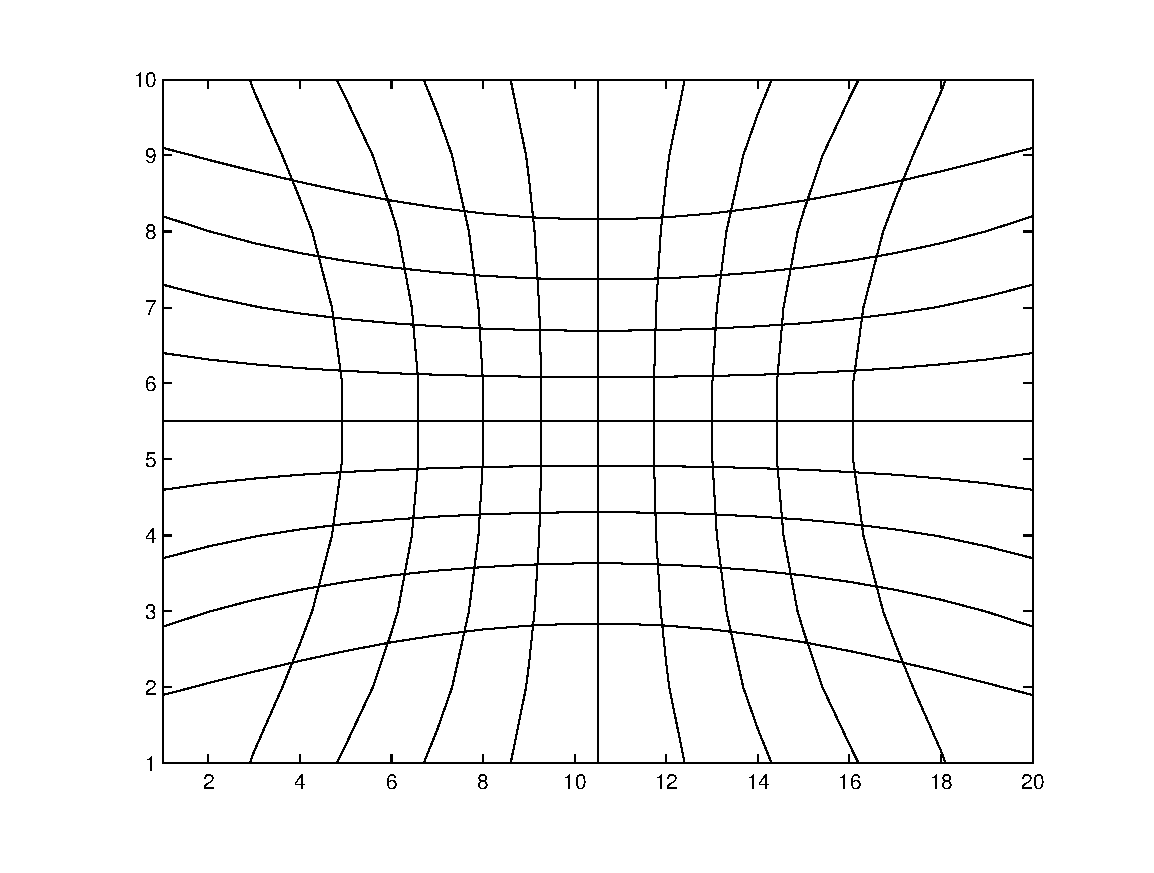
\includegraphics{Harness_ContractedGrid} } &
\scalebox{0.3}{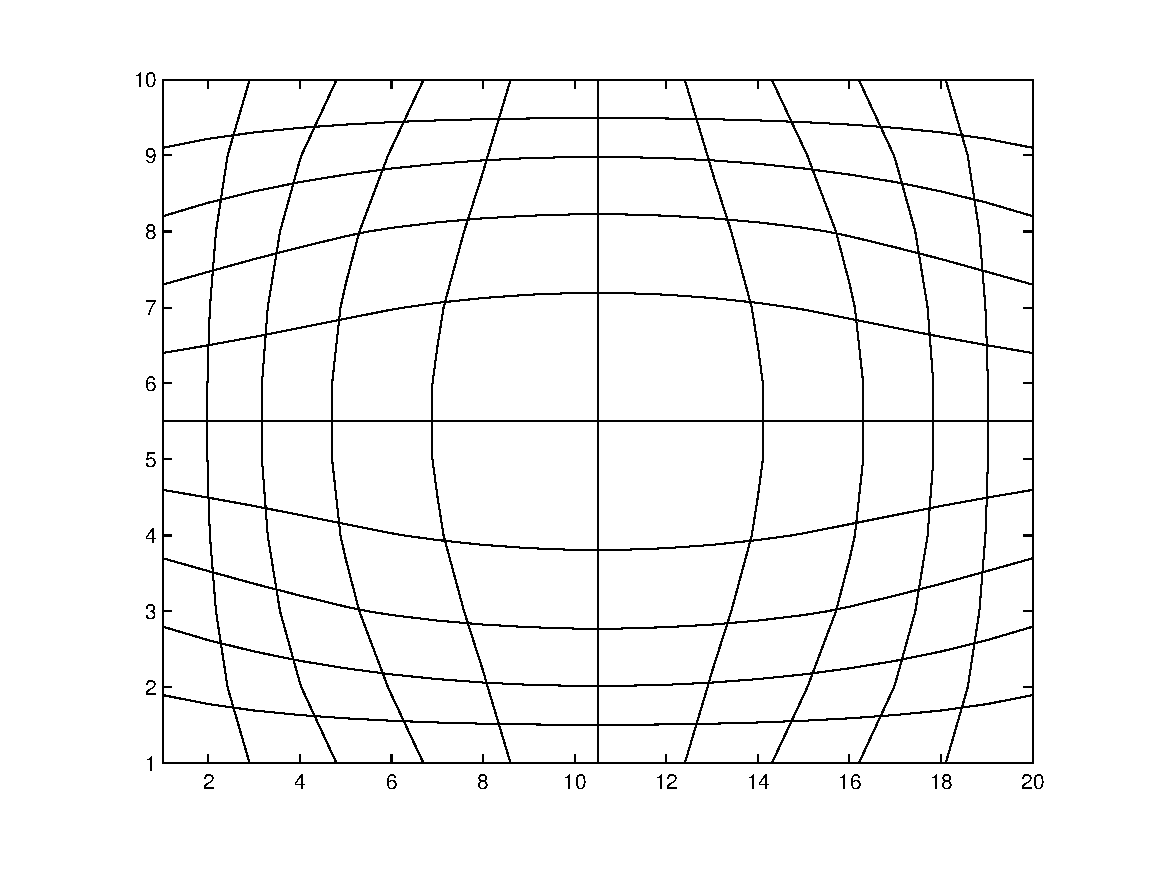
\includegraphics{Harness_ExpandedGrid} } \\
\scalebox{0.3}{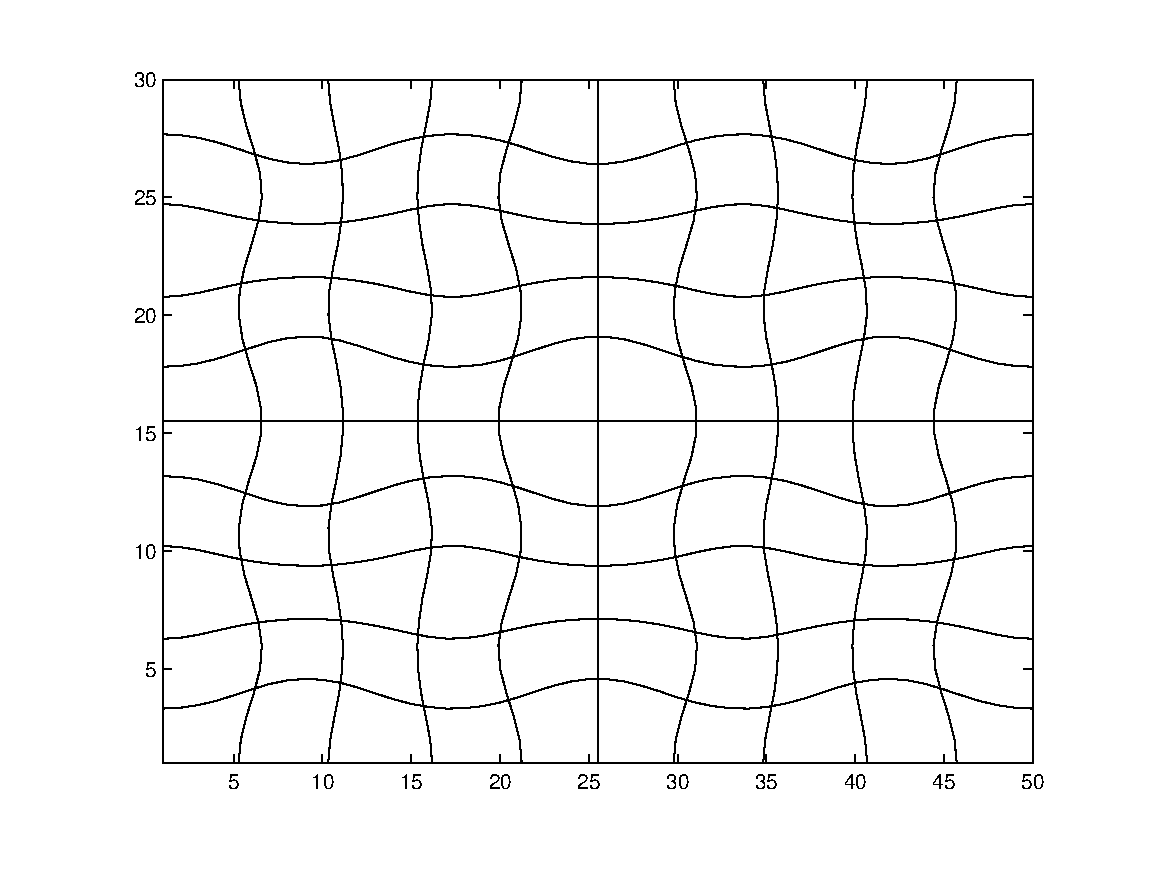
\includegraphics{Harness_SymmetricGrid} } & 
\scalebox{0.3}{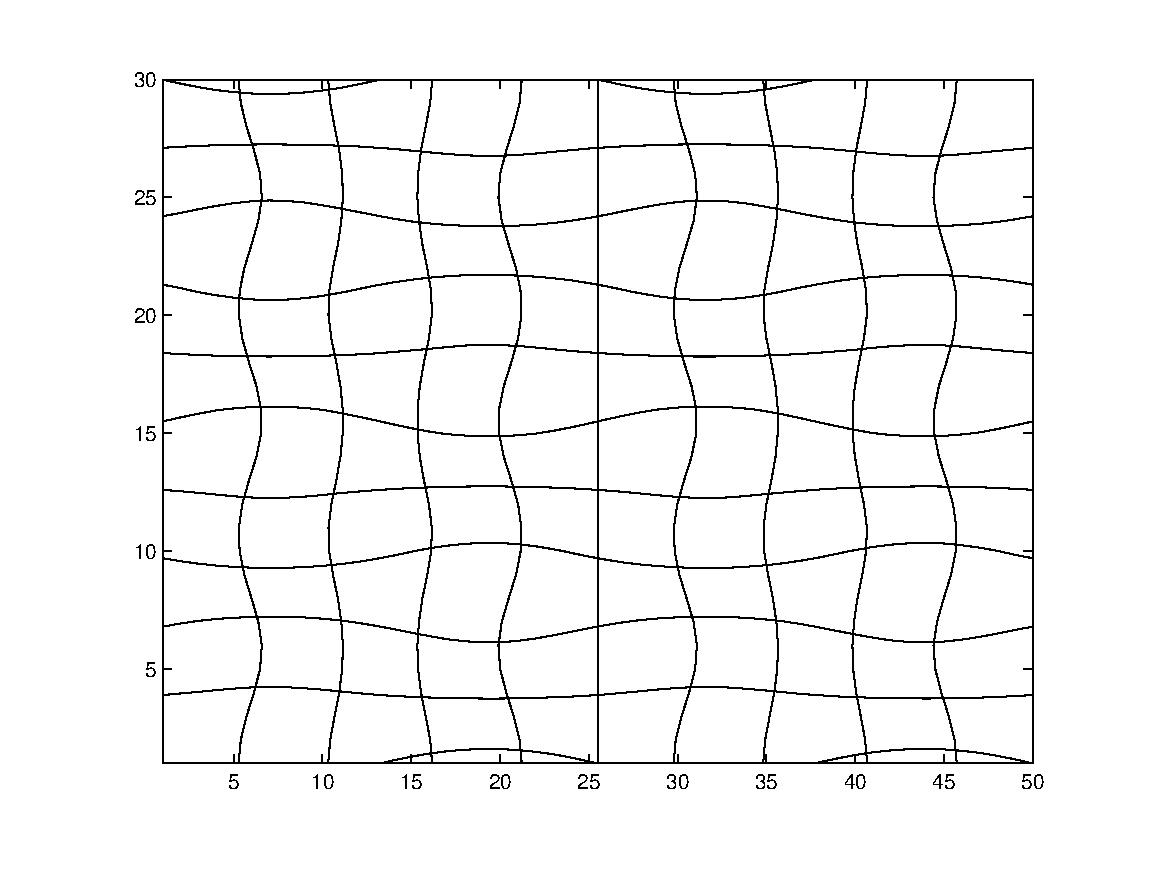
\includegraphics{Harness_AsymmetricGrid} }
\end{tabular}
\caption{The four options for smooth curvilinear grids; clockwise from the top left corner, a contacted grid, an expanded grid, a symmetric sine perturbed grid, and an asymmetric sine perturbed grid.}
\label{fig:harness_smoothGrids}
\end{figure}
\end{center}

This adds up to a total of 2 types of rectilinear grids (uniform and gaussian), each with three options (no connection, spherical pole connection, and a periodic option). A large variety of grids can be formed by mixing and matching the grid types and options. For example a standard latitude-longitude grid on a sphere is formed by using the pair of grid types uniform\_periodic and uniform\_pole. A gaussian grid is formed with uniform\_periodic and gaussian\_pole. And a regional grid on a sphere, without periodicity, with uniform and uniform. A summary of the rectilinear grid types is given below. 
\begin{center}
\begin{tabular}{| c | l |} 
\multicolumn{2}{c}{Rectilinear grid options}  \\ 
\hline
{\em grid type } & {\em modifier} \\
\hline \hline
 UNIFORM &  {\em none } \\ 
              &  \_POLE         \\
              &   \_PERIODIC  \\
 \hline
 GAUSSIAN & {\em none } \\
                 & \_POLE         \\
                &  \_PERIODIC \\
  \hline
\end{tabular}
\end{center}

The various curvilinear grid types are created in the same way of mixing and matching grid type options. A regional expanding grid is formed using the grid types expanding and expanding. Likewise a rotated regional grid is created by
using the grid types rotation\_15degrees and rotation\_15degrees to indicate the grid type. A summary of the curvilinear grid types is given below. 
\begin{center}
\begin{tabular}{| c | l |} 
\multicolumn{2}{c}{Curvilinear grid options}  \\
\hline
{\em grid type } & {\em modifier} \\
\hline \hline
 CONTRACTING & {\em none} \\ 
                    &   \_POLE       \\
                    &   \_PERIODIC  \\
 \hline                   
 EXPANDING  & {\em none} \\ 
                    &   \_POLE       \\
                    &   \_PERIODIC  \\
\hline
SYMMETRIC\_SIN & {\em none} \\ 
                    &   \_POLE       \\
                    &   \_PERIODIC  \\
\hline
ASYMMETRIC\_SIN & {\em none} \\ 
                    &   \_POLE       \\
                    &   \_PERIODIC  \\
\hline
rotation\_15degrees & {\em none} \\ 
\hline
rotation\_30degrees & {\em none} \\ 
\hline
rotation\_30degrees & {\em none} \\ 
\hline 
\end{tabular}
\end{center}
It should be noted that the rotated grid type only supports non-connected domains, and therefore has no option for \_pole and \_periodic connectivity.


%%%%%%%%%%%%%%%%%%%%%%%%%
\paragraph{Specifier file syntax for redistribution}
Since a redistribution test takes either an array or a field and rearranges it in processor space, the test requires only a single grid for the source and destination. The information required is:
\begin{center}
\begin{tabular}{| l |} \hline 
{\em parameters to define a grid for redistribution }  \\
\hline \hline
 Grid rank    \\
 Grid dimensions   \\
 Range of the coordinate axis  \\
 Coordinate units \\
\hline 
\end{tabular}
\end{center}

This is the information is provided by the redistribution grid specifier file.
An example of a redistribution grid specifier file is provided below. 
\begin{center}
\begin{verbatim}
# grid.rc
########################################
map_type: REDISTRIBUTION

# regular rectilinear Grid specification 
map_redist::
#rank spacing  size  range (min/max)  units
#
2  'UNIFORM'  120  -3.14159  3.14159  'RAD'   'UNIFORM'  90  -1.57  1.57  'RAD'   
#
2  'UNIFORM'  400  -180   180  'DEG_E'  'GAUSSIAN'  200 -88   88   'DEG_N'  
::
\end{verbatim}
\end{center}

The first piece of information required for the file is the \texttt{map\_type} key. It should be set to \texttt{REDISTRIBUTION} to indicate that it is intended to define grids for a redistribution test. Next is a configuration table which specifies multiple grids. The specification can be stretched over multiple table lines by use of the continuation symbol $\&$. The order of information is as follows:
\begin{center}
\begin{tabular}{| l |} \hline 
{\em parameters to define a grid for redistribution }  \\
\hline \hline
 Grid rank    \\
 Grid axis type   \\
 Grid size \\
 Range of the coordinate axis  \\
 Coordinate units \\
\hline 
\end{tabular}
\end{center}
 
 There are two 2D grids specified in the file. The first is a standard uniformly spaced latitude-longitude grid, where none of the grid coordinates has any topological connections. The horizontal coordinates are in radians. The second 2D grid is a gaussian spherical grid. The gaussian grid has a spherical topology and is in degrees. 
 
Four types of coordinate units are supported; degrees, radians, meters and kilometers.  Each has multiple equivalent key words. 
 \begin{center}
\begin{tabular}{| l | l |} 
\multicolumn{2}{c}{ Supported units }  \\
\hline 
{\em name } & {\em key word} \\
\hline \hline
Degrees & DEGREES \\
  & DEG \\
  & DEG\_E \\
  & DEG\_N \\
  \hline
Radians & RADIANS \\
  & RAD \\
  \hline
 Meters & METERS \\
    & M \\
    \hline
   Kilometers & KILOMETERS \\
      & KM \\
\hline 
\end{tabular}
\end{center}


%%%%%%%%%%%%%%%%%%%%%%%%%
\paragraph{Specifier file syntax for regridding}
The process of regridding takes a distributed test field from a source grid and interpolates it to a distributed destination grid. Therefore it requires information specifying both a source and destination grid, and an explicit test function to interpolate. The information required is:
\begin{center}
\begin{tabular}{| l |} \hline 
{\em parameters to define a grid for remapping }  \\
\hline \hline
 source and destination grid rank    \\
 source and destination grid axis type   \\
 source and destination grid dimensions   \\
 source and destination range of coordinate axis  \\
 source and destination coordinate units \\
 test function with parameters to interpolate \\
\hline 
\end{tabular}
\end{center}

This information is provided by the regridding grid specifier file.
An example of a regridding grid specifier file is provided below. 
\begin{center}
\begin{verbatim}
# grid.rc
########################################
map_type: REGRID

################################################################################
# grid | source | grid    |    grid   | grid  | units | destination | 
# rank |  tag   | spacing | dimension | range |       |    tag      |
################################################################################
# Grid specification for regridding

#rank spacing  size  range (min/max)  units
map_regrid::
# example of a pair of 2D periodic grids 
2   SRC    UNIFORM_PERIODIC   120   -3.14159  3.14159  RADIANS   
&              UNIFORM_POLE             90    -1.57        1.57        RADIANS   
&   DST    UNIFORM_PERIODIC   120  -180      180             DEG_E   
&              GAUSSIAN_POLE           88    -88        88             DEG_N   
&   FUNCTION    CONSTANT   2.1 0.1  END
::
\end{verbatim}
\end{center}

The first piece of information required for the file is the \texttt{map\_type} key. It should be set to \texttt{REGRID} to indicate that it is intended to define grids for a regridding test. Next is a configuration table which specifies multiple pairs of grids. The specification can be stretched over multiple table lines by use of the continuation symbol $\&$. The order of information is as follows:
\begin{center}
\begin{tabular}{| l |} \hline 
{\em parameters to define a grid for reremapping }  \\
\hline \hline
 Grid rank    \\
 Source grid axis type   \\
 Source grid size \\
 Source range of the coordinate axis  \\
 Source coordinate units \\
 Destination grid axis type   \\
 Destination grid size \\
 Destination range of the coordinate axis  \\
 Destination coordinate units \\
 Test function and parameters \\
\hline 
\end{tabular}
\end{center}

The regridding grid specifier file contains a pair of 2D grids. The source grid is a standard latitude-longitude grid on a spherical topology. The destination grid is a spherical gaussian grid also on a spherical topology. The source grid is in radians, while the destination grid is in degrees. The test function is a periodic function of the grid coordinates. 

The one new piece of information for the regridding specifier files are the predefined test functions. The test functions provide a physical field to be interpolated and are generated as an analytical function of the grid coordinates. Supported options include:
\begin{center}
\begin{tabular}{| l | l | l |} 
\multicolumn{2}{c}{ Test functions }  \\
\hline 
{\em name } & {\em function} & {\em parameters} \\
\hline \hline
constant & set value at all locations & value, relative error \\
coordinate & set to a multiple of the coordinate values & scale, relative error \\
spherical harmonic & periodic function of the grid coordinates & amplitudes and phases, relative error \\
\hline 
\end{tabular}
\end{center}

The CONSTANT value test function sets the field to the value of the first parameter following the name. The second value is the relative error threshold. For example, the test function specification:

\begin{center}
\begin{verbatim}
&   FUNCTION    CONSTANT   2.1 0.1  END
\end{verbatim}
\end{center}

indicates that the field is set to the constant value of $2.1$, with a relative error threshold 
of $0.1$. This test function specification holds for grids of any rank. 

The COORDINATE test function sets the field to the value of the one of the grid coordinates multiplied by the value of the first parameter following the name. The second value is the relative error threshold. For example, the test function specification:

\begin{center}
\begin{verbatim}
&   FUNCTION    COORDINATEX   0.5 0.1  END
\end{verbatim}
\end{center}

indicates that the field is set to one half of the X coordinate values. For a 2D grid the coordinate options include COORDINATEX and COORDINATEY. For a 3D grid there is the additional option of COORDINATEZ. Again, the relative error threshold is $0.1$.
This test function specification holds for grids of any rank. 

The SPHERICAL\_HARMONIC test function sets the field to the periodic harmonic function 
$|a+b| + a*\cos(2\pi * k_x * x/L_x ) + b*\sin(2\pi * l_y * x/L_y )$.
The parameters follow the order

\begin{center}
\begin{verbatim}
&   FUNCTION    SPHERICAL_HARMONIC  a   kx  b   ly    rel_error  END
\end{verbatim}
\end{center}

This test function specification is only valid for 2D grids.     





%%%%%%%%%%%%%%%%%%%%%%
\subsubsection{Distribution Specification}
\label{sec:harness_distributionsspecifier}
The purpose of the distribution specification is to characterize the distribution of the grid. It differs from the grid specification in that it is designed to specify the distribution as both absolute values such as $2 \times 3$ PETS as well as in relative terms based on fractions of the total number of PETS. This second option is intended to allow the distribution space to scale with changing machine resources without having to change the distribution specification file. 

Here is an example of a distribution specification file for block and block cyclic distributions.
\begin{center}
\begin{verbatim}
##################################################
# descriptive | source | source | operator | destination | dest | operator | end
# string      |  tag   |  rank  |  & value |     tag     | rank | & value  | tag
##################################################

# table specifing 2D to 2D distributions
distgrid_block_2d2d::

# example with two fixed distribution sizes
 '(1,2)-->(2,1)'  'SRC' 2  'D1==' 1  'D2==' 2  'DST' 2  'D1==' 2  'D2==' 1  'END'  

# example with one fixed and one variable distribution size
 '(1,n)-->(n,1)'  'SRC' 2  'D1==' 1  'D2=*' 1  'DST' 2  'D1=*' 1  'D2==' 1  'END'  

# example with variable distribution sizes
 '(2n,n/2)-->(n/2,2n)'  'SRC'  2  'D1=*'  2    'D2=*'  0.5  
 &                      'DST'  2  'D1=*'  0.5  'D2=*'  2     'END'

# another example with variable distribution sizes
 '(2n,n/2)-->(2n,(n/2)-1)'  'SRC' 2  'D1=*' 2  'D2=*'  0.5  
 &                          'DST' 2  'D1=*' 2  'D2=*'  0.5  'D2=+' 1   'END'
::

# table specifing 3D to 3D distributions
distgrid_block_3d3d::

# example with two fixed distribution sizes
 '(1,2,1)-->(2,1,1)'  'SRC' 3  'D1==' 1  'D2==' 2  'D3==' 1  
 &                    'DST' 3  'D1==' 2  'D2==' 1  'D3==' 1  'END'  
::
\end{verbatim}
\end{center}
The contents of the file are tables which specify pairs of distributions. Each table specifies a particular rank of distributions. The first table consists of 2D to 2D distributions, while the second table consists of a 3D to 3D pair of distributions. 
The order of information is as follows:
\begin{center}
\begin{tabular}{| l |} \hline 
{\em parameters to define a grid distribution }  \\
\hline \hline
 Descriptive string    \\
 Source key   \\
 Source distribution rank \\
 Source distribution axis and size for each dimension of the distribution  \\
 Destination key \\
 Destination distribution rank    \\
 Destination grid size \\
 Destination distribution axis and size for each dimension of the distribution  \\
 Termination key \\
\hline 
\end{tabular}
\end{center}
The first example in the table starts with a string used by the report as a brief description of the distribution. Such as  $(1,2)-->(2,1)$ which indicates a source distribution of $ 1 \times 2$ and a destination distribution of $ 2 \times 1$. Next comes a key word, either \texttt{SRC} or \texttt{DST} to indicate the beginning of the source and destination descriptions, respectively. Following each tag is a specification of the distribution. In the first case a fixed source distribution is specified by the entries $D1==1$ and $D2=2$. This indicates that the source distribution is fixed to be $ 1 \times 2$, provided that the test is running with at least two processors. Likewise the destination distribution is fixed to $ 2 \times 1$.

The second example, illustrates how to indicate a scalable distribution. Again the entry $D1==1$ indicates that the first dimension of the distribution is set to one, but the entry $D2=*1$ has a different meaning. It takes the total number of PETS NPETS and scales it by one. Therefore the source distribution becomes $ 1 \times NPETS$. It automatically scales with the number of PETS. Likewise, the destination distribution is set to $NPETS \times 1$. 

The third example is completely dynamic. Since both $D1$ and $D2$ are scalable, each dimension starts with $N$ PETS, where $N$ is the square root of $NPETS$ rounded down to the nearest integer. Therefore $N\times N \leq NPETS$. So if $NPETS=4$, Then $N=2$. If $NPETS=6$ then $N$ still equals $4$. This base value is then modified by the indicated entries. In this case the source distribution is $2 N \times 1/2 N$, since the tag $D1=*  2$ indicates that first dimension is the result of the base value being multiplied by two, and the second dimension is the result of the base value being multiplied by one half. Likewise, the destination distribution is set to $1/2 N \times 2N$, no matter the number of $NPETS$.

For a rank three scalable distribution, $N$ is the cube root of NPETS rounded down to the next integer. And so on for higher rank distributions. 

The fourth example illustrates the last option in the syntax. Again, since the distribution specifies two scalable distributions, $N$ is the square root of $NPETS$ rounded down to the nearest integer. The source distribution is exactly the same as in the third example, but destination distribution has a new entry $D2=+ 1$. The first dimension of the destination distribution is set to $2N$ by the entry $D1=* 2$. the second dimension is first set to $1/2N$ by the entry $D2=* 0.5$, but then modified further to $(1/2)(N) +1$ by the entry $D2=+ 1$. The resulting destination distribution is $2N \times (1/2)(N) +1$. 

The syntax for modifying the size of the distribution space combines according to the order of the operations. The entries $D2=* 0.5$ and $D2=+ 1$, are not identical to $D2=+ 1$ and $D2=* 0.5$, which would result in a dimension of size $(1/2)(N+1)$.

Three operations are supported:
\begin{center}
\begin{tabular}{| c | c |} \hline 
{\em Distribution specification operations}  \\
\hline \hline
 D\# == & specify a fixed value \\
 D\# =* & multiply a base value by a constant \\
 D\# =+ & add a constant to the base value  \\
 \hline 
\end{tabular}
\end{center}

%%%%%%%%%%%%%%%%%%%%%%
\subsubsection{Class Specification}
The class specific specifier file is current unused, but is made available for future test expansion.


%%%%%%%%%%%%%%%%%%%%%%
%%%%%%%%%%%%%%%%%%%%%%
\subsection{Reporting test results}
The test harness offers the option of producing a human readable report on the test results. The report consists of a concise summary of the test configuration along with the test results. The test configuration is described in terms of the Field Taxonomy syntax and user provided strings. The intent is not to provide a exhaustive description of the test, but rather to provide a useful description of the failed tests.

Consider a problem descriptor string consisting of two descriptor strings describing an ensemble of remapping tests. 
\begin{center}
\begin{verbatim}
[ B1 G1; B2 G2 ] =C=> [ B1 G1; B2 G2 ] @{+,+}
[ B1 G1; B2 G2 ] =B=> [ B1 G1; B2 G2 ] @{+,+} 
\end{verbatim}
\end{center}

Suppose the associated specifier files indicate that the source grid is rectilinear and is 100 X 50 in size. The destination grid is also rectilinear and is 80 X 20 in size. The remapping is conducted from the A-grid position of the source grid to the B-grid stagger of the destination grid. Both grids are block distributed in two ways, 1 X NPETS and NPETS X 1. And suppose that the first dimension of both the source and destination grids are periodic. If the test succeeds for the conservative remapping, but fails for one of the first order bilinear remapping configurations, the reported results
could look something like
\begin{center}
\begin{verbatim}
SUCCESS: [B1 G1; B2 G2 ] =C=> [B1 G1; B2 G2 ] @{+,+}
FAILURE: [B1{1} G1{100}+P; B2{npets} G2{50} ] =B=> 
                         [B1{1} G1{80}+P; B2{npets} G2{20} ] @{+,+}
     failure at line 101 of test.F90
SUCCESS: [ B1{npets} G1{100} +P; B2{1} G2{50} ] =B=> 
                         [ B1{npets} G1{80}+P; B2{1} G2{20} ] @{+,+}
\end{verbatim}
\end{center}
Notice that the problem descriptor string differs from that of the configuration files. This is because it represents specific realizations of ensemble. For example 
\begin{center}
\begin{verbatim}
[ B1{npets} G1{80}+P; B2{1} G2{20} ] @{+,+}
\end{verbatim}
\end{center}
indicates that the 2D block of memory is periodic in the first dimension by the addition of the $+P$ to the first grid key. The size of the grid is indicated as $80 \times 20$ by the size arguments appended to the grid indicators $G1 \{80 \}$ and $G2 \{ 20 \}$. The size of the distribution is indicated in the same way as $npets \times 1$ by the block distribution indicators $B1 \{ npets \}$ and $B2 \{ 1 \}$.

The report indicates that all the test configurations for the conservative remapping are successful. This is indicated by the key word SUCCESS which is followed by the successful problem descriptor string. Since all of the tests in the first case pass,there is no need to include any of the specifier information. For the second ensemble of tests, one configuration passed, while the other failed. In this case, since there is a mixture of successes and failures, the report includes specifier information for all the configurations to help indicate the source of the test failure. 


The supplemental information, while not a complete problem description, since it lacks items such as the physical coordinates of the grid and the nature of the test field, includes information crucial to isolating the failed test.





